\documentclass[tikz,border=8pt]{standalone}
% Shared look for every TikZ diagram. Load with \input{../../tools/tikz-style.tex}
\usepackage[T1]{fontenc}
\usepackage{lmodern}
\renewcommand{\sfdefault}{lmr}  % diagrams use the same serif as the text
\usetikzlibrary{arrows.meta, positioning, shapes.geometric, calc, fit, backgrounds}
\definecolor{cblue}{HTML}{4C78A8}
\definecolor{corange}{HTML}{F58518}
\definecolor{cgreen}{HTML}{54A24B}
\definecolor{cred}{HTML}{E45756}
\definecolor{cpurple}{HTML}{B279A2}
\definecolor{cgrey}{HTML}{6B6B6B}
\tikzset{
  every picture/.style={font=\sffamily, line width=1.2pt},
  box/.style={draw=#1, fill=#1!12, rounded corners=4pt, align=center, inner sep=7pt, minimum height=1.1cm},
  box/.default=cgrey,
  arrow/.style={-{Stealth[length=3mm]}, draw=cgrey, line width=1.4pt},
  title/.style={font=\sffamily\bfseries\Large},
  note/.style={font=\sffamily\small, text=cgrey, align=center},
}
\AtBeginDocument{\hyphenpenalty=10000 \exhyphenpenalty=10000}

\newcommand{\cell}[4]{\node[draw=cgrey, line width=0.8pt, minimum width=1.25cm, minimum height=0.95cm, fill=#4, font=\sffamily] at ({#1},{#2}) {#3};}
\begin{document}
\begin{tikzpicture}
  \node[title, anchor=west] at (-0.6,1.2) {$\partial L/\partial W_1$ = input $X$ convolved with $\partial L/\partial Z_1$};
  \foreach \r in {1,2,3}{\foreach \c in {1,2,3}{
    \pgfmathtruncatemacro{\on}{(\r<3)*(\c<3)}
    \ifnum\on=1 \cell{(\c-1)*1.25}{-(\r-1)*0.95}{$x_{\r\c}$}{cblue!22}\else \cell{(\c-1)*1.25}{-(\r-1)*0.95}{$x_{\r\c}$}{white}\fi
  }}
  \draw[corange, line width=2pt] (-0.625,0.475) rectangle (1.875,-1.425);
  \node[below] at (1.25,-2.5) {input $X$, $3 \times 3$};
  \node at (4.2,-0.95) {\huge $*$};
  \foreach \r in {1,2}{\foreach \c in {1,2}{
    \cell{5.2+(\c-1)*1.25}{-0.475-(\r-1)*0.95}{\scriptsize$\partial L/\partial z_{\r\c}$}{corange!22}
  }}
  \node[below] at (5.825,-2.5) {$\partial L/\partial Z_1$, $2 \times 2$};
  \node at (8.0,-0.95) {\huge $=$};
  \foreach \r in {1,2}{\foreach \c in {1,2}{
    \cell{9.2+(\c-1)*1.25}{-0.475-(\r-1)*0.95}{\scriptsize$\partial L/\partial w_{\r\c}$}{cgreen!22}
  }}
  \node[below] at (9.825,-2.5) {$\partial L/\partial W_1$, $2 \times 2$};
  \node[anchor=west, align=left] at (-0.6,-4.0) {top-left entry: lay $\partial L/\partial Z_1$ on the highlighted window of $X$, multiply cell by cell, add:\\[3pt]
    $\dfrac{\partial L}{\partial w_{11}} = \dfrac{\partial L}{\partial z_{11}}x_{11} + \dfrac{\partial L}{\partial z_{12}}x_{12} + \dfrac{\partial L}{\partial z_{21}}x_{21} + \dfrac{\partial L}{\partial z_{22}}x_{22}$};
\end{tikzpicture}
\end{document}
